\chapter{Integration of the FCN into the original work of Egger et al}

The aim of this chapter is to combine the advantages of the iterative segmentation method of Egger et al and of the segmentation by the FCN. In the previous chapters, we saw that both approaches have their strengths. Let us summarise them:

\begin{itemize}[nolistsep]
	\item Strengths of the segmentation of the FCN:
	\begin{itemize}[nolistsep]
		\item Although the borders of the segmentation are sometimes a bit fuzzy, almost only skin pixels are segmented (very few false positives).
		\item As long as the face is not rotated (roll rotation), the FCN is very sturdy against variations in pitch and yaw.
		\item Even if the occlusion has approximately the same colour as the face, the FCN may recognises the occlusion [Figure \ref{fig:chap3:zlabelsandfits}].
	\end{itemize}
	\item Strengths of the segmentation of Egger et al
	\begin{itemize}[nolistsep]
		\item It is an iterative algorithm, the segmentation is always updated, based on the ever-changing 3DMM fit.
		\item The algorithm can find occlusions that are thin and small, and the borders of the segmentation are very sharp [\Cref{fig:chap4:harry}].
		\item Egger et al use a beard prior to exclude beards from the segmentation [\Cref{fig:chap4:Beard_Prior_example}].
	\end{itemize}
\end{itemize}

\begin{figure}[H]
	\centering
	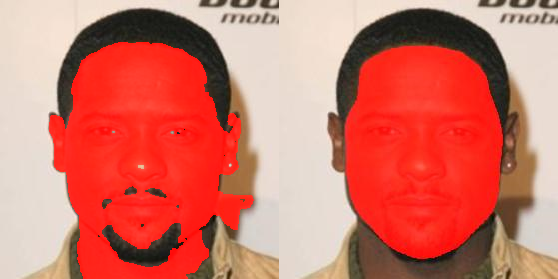
\includegraphics[width=.33 \textwidth]{Figures/chap4/Beard_Prior_example.png}
	\caption{On the left-hand side, the segmentation of Egger which excludes the beard from the segmentation (but oversegments the face). The right-hand side shows the same target image overlaid with the segmentation of the FCN.}
	\label{fig:chap4:Beard_Prior_example}
\end{figure}

We combined both approaches so that the fitting algorithm of Egger et al takes the segmentation of the FCN as the initial mask and refines it during the following iterations. The biggest weakness of the FCN is its inability to detect small or thin occlusions [\Cref{fig:chap4:harry}]. 

\begin{figure}
\begin{center}
\newcolumntype{C}{>{\centering\arraybackslash} m{2.4cm} }  %# New column type
\begin{tabular}{m{1.3cm}|SC|SC}
	& EGGER & FCN \\ \hline
	z-labels & \subfloat{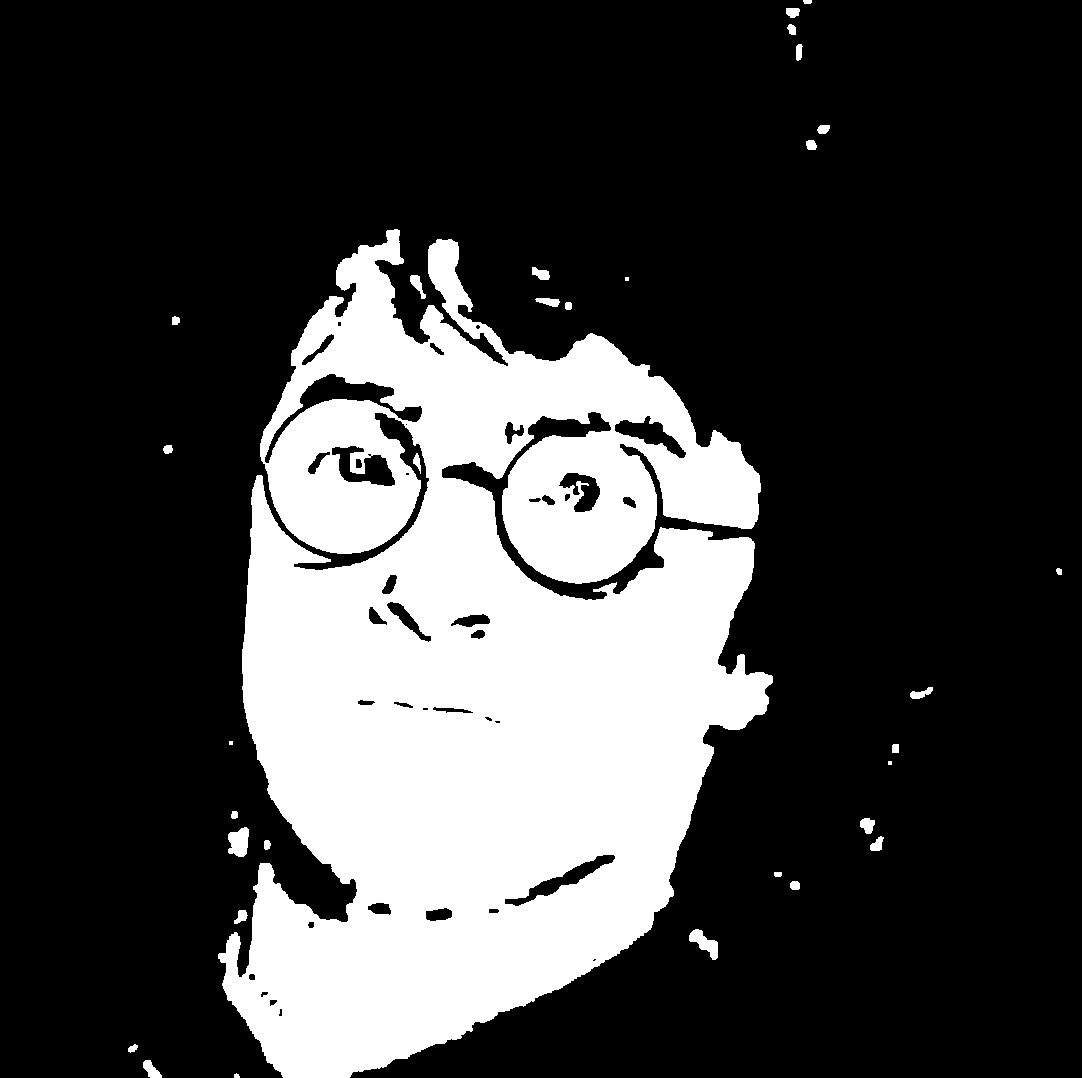
\includegraphics[width=0.16\textwidth]{Figures/chap4/harry_mask_EGGER_.png}} &
	\subfloat{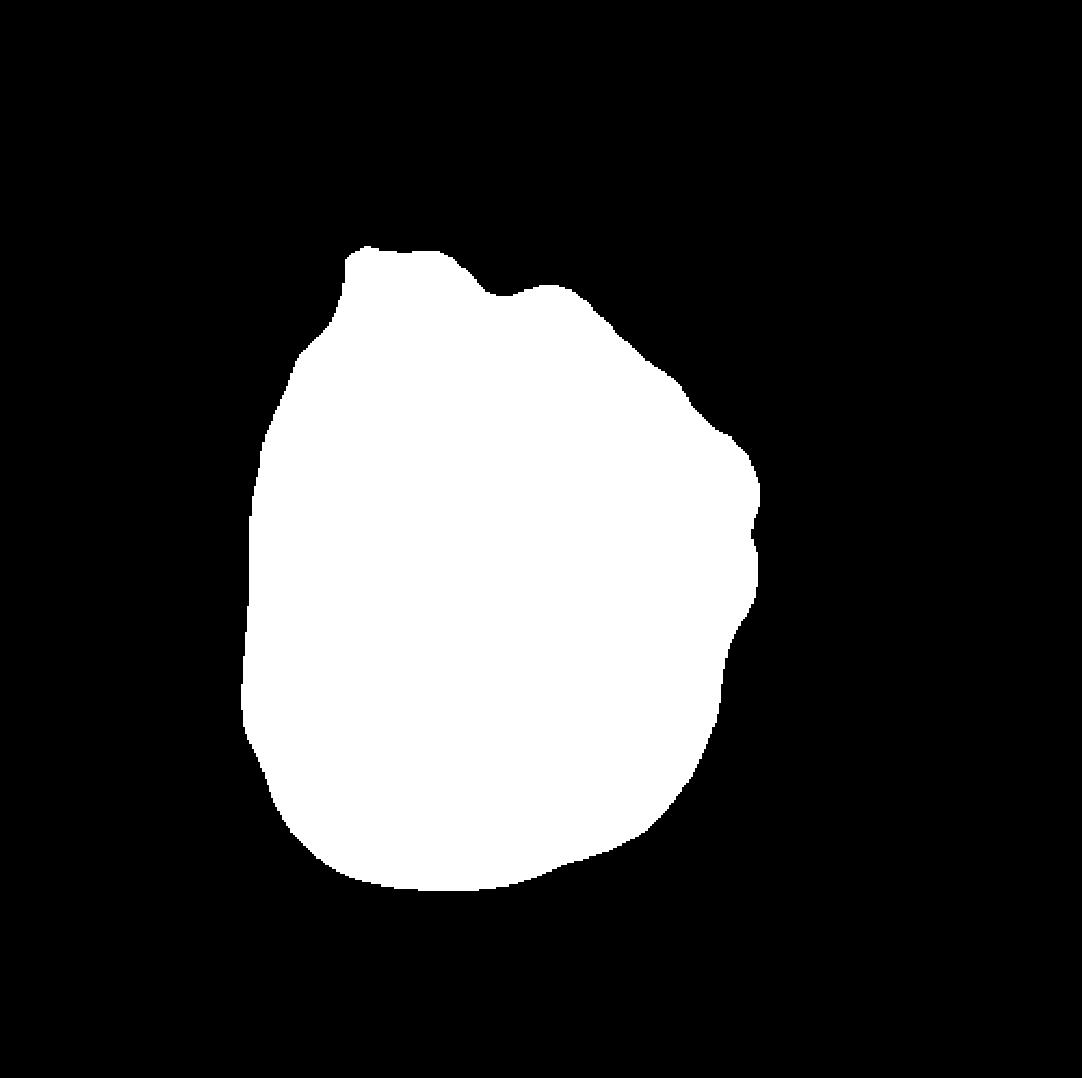
\includegraphics[width=0.15\textwidth]{Figures/chap4/harry_mask_FCN_.png}}\\ \hline
	fits & \subfloat{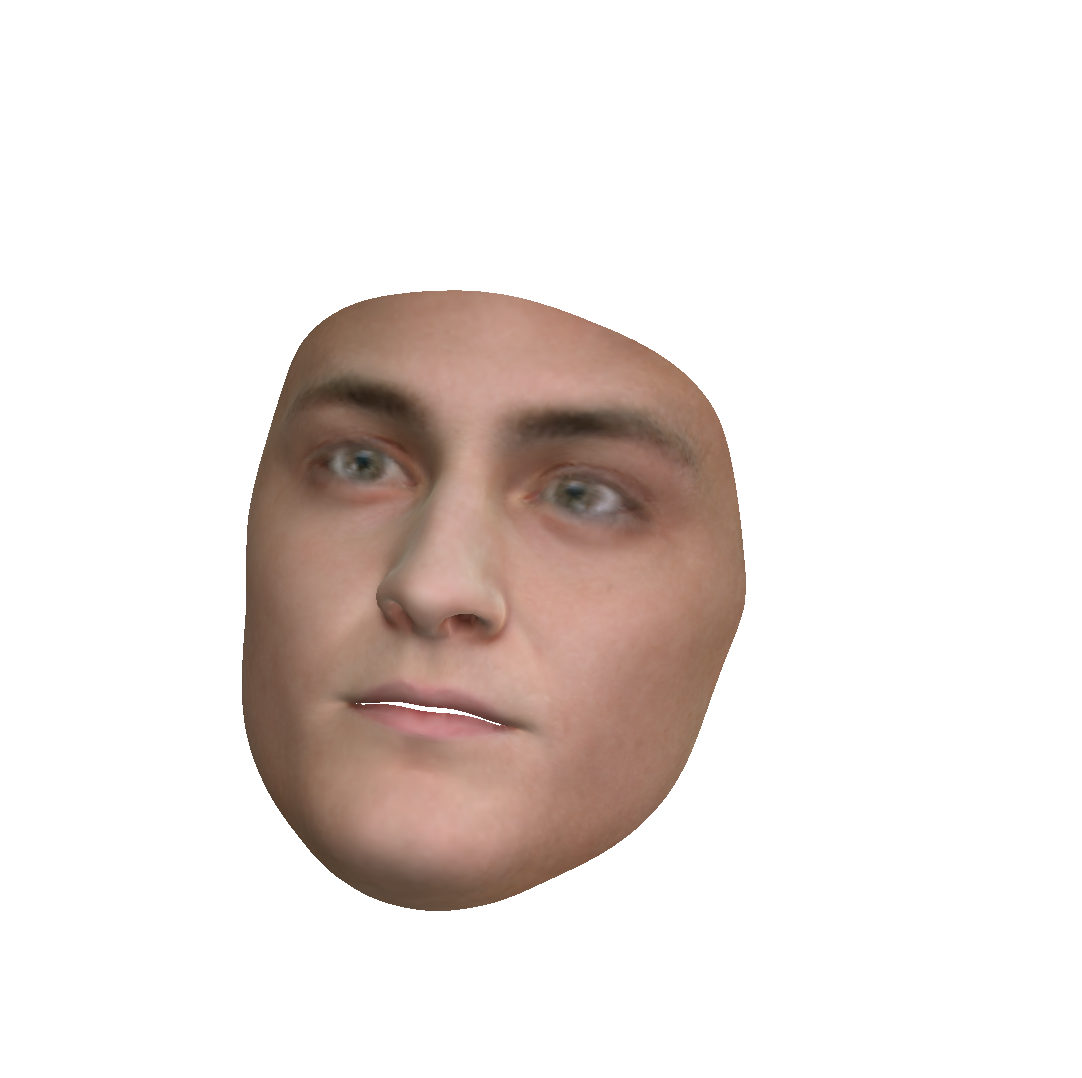
\includegraphics[width=0.16\textwidth]{Figures/chap4/harry_fit_EGGER.png}} & 
	\subfloat{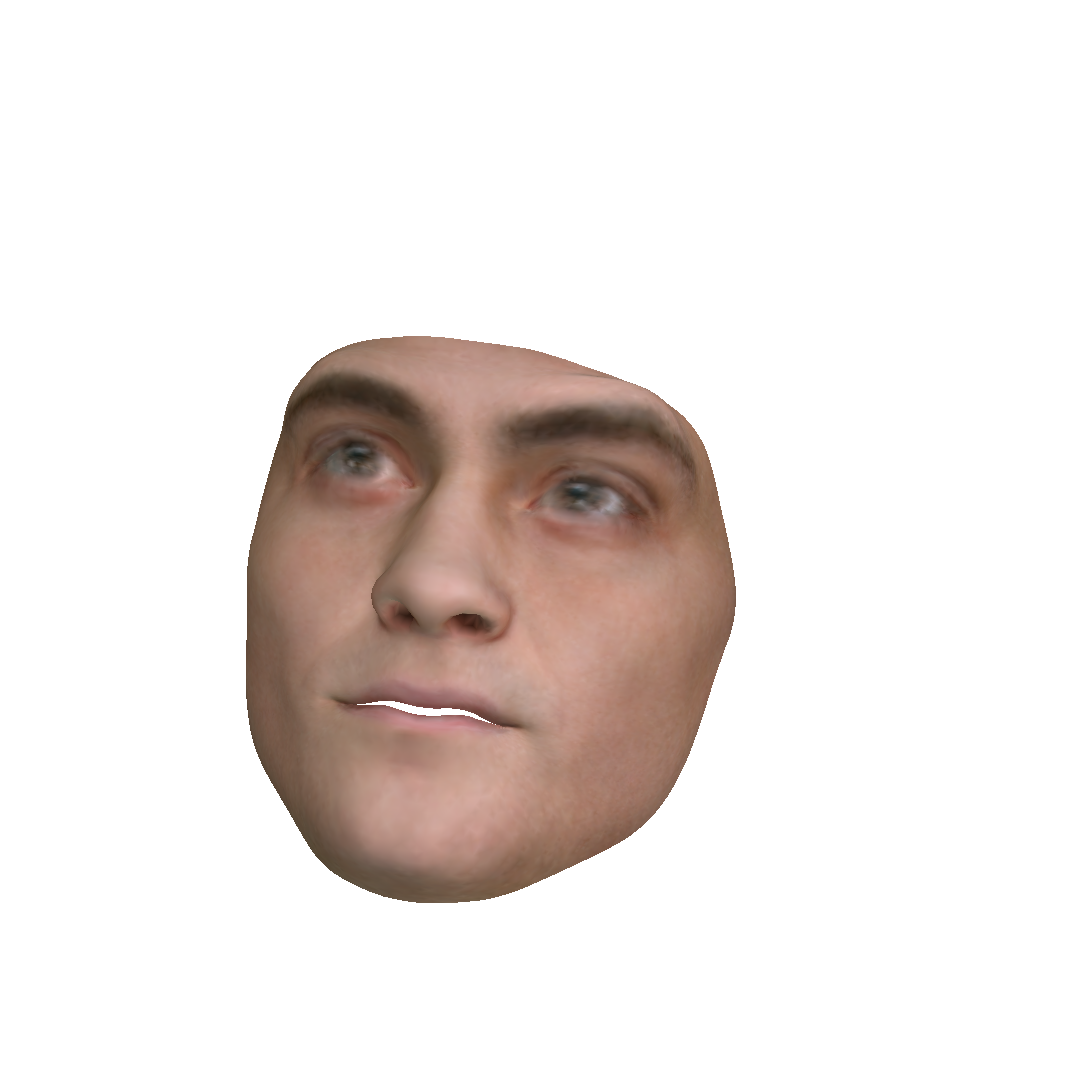
\includegraphics[width=0.16\textwidth]{Figures/chap4/harry_fit_FCN.png}} \\
\end{tabular}
\caption{This example illustrates a major advantage and a disadvantage of Egger's approach. The FCN can't find the thin glasses but segments the eyes as face while Egger does not.}
\label{fig:chap4:harry}
\end{center}
\end{figure}

It is precisely this weakness of the FCN that is a strength of the approach of Egger et al. It is therefore very suitable to take the FCN's mask as a first segmentation, which contains almost only facial pixels and then refine this segmentation and search for thin occlusions by applying the occlusion-aware segmentation method of Egger to it.\\
\\
However, our assumption is that the final segmentation does not differ much from the mask according to Egger et al alone because of the Metropolis-Hastings sampling in every iteration. The random walk always ends in the same region, regardless of the starting point.\\
\\
We first show an example with a tailored (face12) target face [\Cref{fig:chap4:bsp1} and \Cref{fig:chap4:fit_comparison_1}], then an example where the target face is a 'bfm'-Version face [\Cref{fig:chap4:bsp2} and \Cref{fig:chap4:fit_comparison_2}]. \\
\\
Both experiments in this chapter show that the error of a fit with a combined mask is very close to the error of a fit with the iterative segmentation of Egger et al. It is interesting that the model parameters get a little better with the combined segmentation but the lighting gets worse in both cases.\\

\pagebreak

\section{Evaluation on the Tailored Face}
In the following experiment, we use a 'face12'-version rendering of a face as input for the fit. The facial image which should be modelled is usually called the \textit{target image}.
\begin{figure}
\centering
\subbottom[initial mask of the FCN]{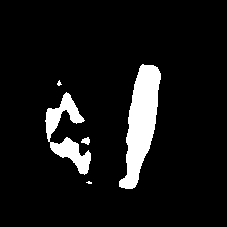
\includegraphics[width=0.24\textwidth]{Figures/chap3/hands_test6_mask_FCN.png}\label{fig:chap4:bsp1_mask_FCN}}
\subbottom[segmentation of Egger et al]{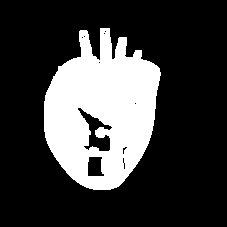
\includegraphics[width=0.24\textwidth]{Figures/chap3/hands_test6_mask_EGGER.png}\label{fig:chap4:bsp1_mask_EGGER}}
\subbottom[combined segmentation]{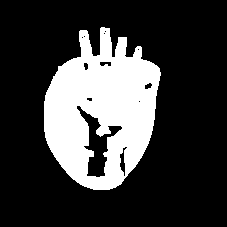
\includegraphics[width=0.24\textwidth]{Figures/chap4/test6_mask_combined.png}\label{fig:chap4:bsp1_mask_combined}}
\subbottom[fit with the combined mask (Subfigure (c))]{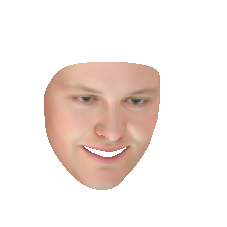
\includegraphics[width=0.24\textwidth]{Figures/chap4/test6_fit_combined.png}\label{fig:chap4:bsp1_fit_combined}}
\caption{An example of the combination of the two masks. [Figure \ref{fig:chap4:bsp1_mask_FCN}] shows the segmentation of the FCN while [Figure \ref{fig:chap4:bsp1_mask_EGGER}] shows the segmentation by Egger et al. The combination is depicted in [Figure \ref{fig:chap4:bsp1_mask_combined}]. The target image for this example is the same as in [Figure \ref{fig:chap3:hands_PARAMETRIC}]. We see our suspicion that the initial segmentation only makes a tiny difference confirmed. [Figure \ref{fig:chap4:bsp1_fit_combined}] shows the resulting fit with the combined mask.}
\label{fig:chap4:bsp1}
\end{figure}

\pgfplotsset{height=7.5cm,width=8.5cm,compat=1.9}
\begin{figure}
	\begin{center}
		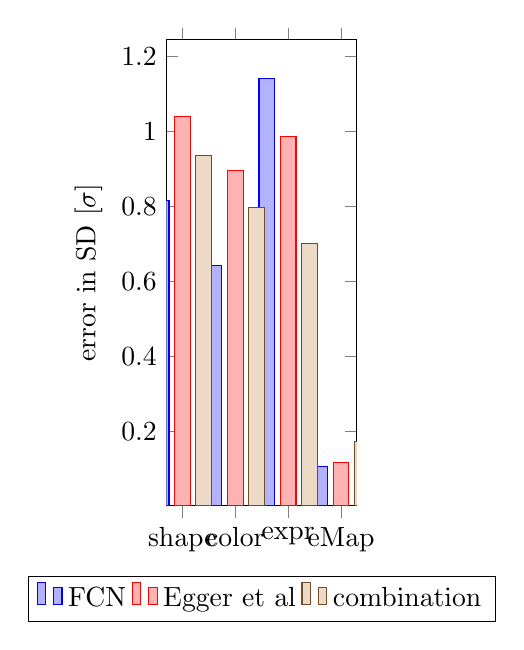
\begin{tikzpicture} 
		\begin{axis}[ 
		ybar,
		bar width=0.2cm,
		enlargelimits=0.1, 
		legend style={at={(0.5,-0.15)}, anchor=north,legend columns=-1}, 
		ylabel={error in SD [$\sigma$]},
		symbolic x coords={shape,color,expr,eMap}, 
		xtick=data,
		%nodes near coords, 
		%nodes near coords align={vertical}, 
		] 
		
		\addplot coordinates {(shape,0.8148) (color,0.6424) (expr,1.1412) (eMap,0.1045)}; 
		\addplot coordinates {(shape,1.0404) (color,0.8947) (expr,0.9855) (eMap,0.1156)}; 
		\addplot coordinates {(shape,0.9369) (color,0.7965) (expr,0.6999) (eMap,0.1715)}; 
		
		\legend{FCN, Egger et al, combination}
		\end{axis} 
		\end{tikzpicture}
		\pgfplotsset{height=7.5cm,width=4cm,compat=1.9}
		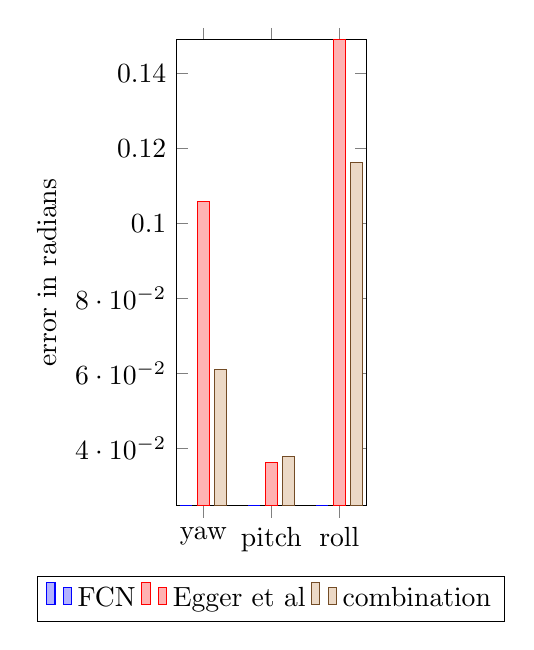
\begin{tikzpicture} 
		\begin{axis}[ 
		ybar,
		bar width=0.15cm,
		%enlarge limits=0.05,
		enlarge y limits=0.00,
		enlarge x limits=0.2,
		legend style={at={(0.5,-0.15)}, anchor=north,legend columns=-1}, 
		ylabel={error in radians},
		symbolic x coords={yaw,pitch,roll}, 
		xtick=data,
		] 
		
		\addplot coordinates {(yaw,0.0247) (pitch,0.0247) (roll,0.0247)}; 
		\addplot coordinates {(yaw,0.1059) (pitch,0.0362) (roll,0.1489)}; 
		\addplot coordinates {(yaw,0.0611) (pitch,0.0379) (roll,0.1163)}; 
		
		\legend{FCN, Egger et al, combination}
		\end{axis} 
		\end{tikzpicture}
	\end{center}
	\caption{A comparison of the Basel Face Model parameters. In this plot, the fits with the masks of Egger, of the FCN [Figure \ref{fig:chap3:zlabelsandfits}], and with the combined mask [\Cref{fig:chap4:bsp1_fit_combined}] are compared. Per parameter, only the first 5 dimensions are considered. In all considered Basel Face Model parameters (shape, color, and expression), the version with the combined mask has a lower error than the slower fit with the mask of Egger et al alone.}
	\label{fig:chap4:fit_comparison_1}
\end{figure}

\begin{figure}
	\centering
	\subbottom[Egger et al]{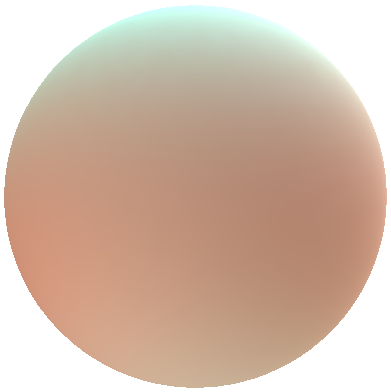
\includegraphics[width=0.2\textwidth]{Figures/chap4/illuminations/test6_EGGER.png}}
	\subbottom[FCN]{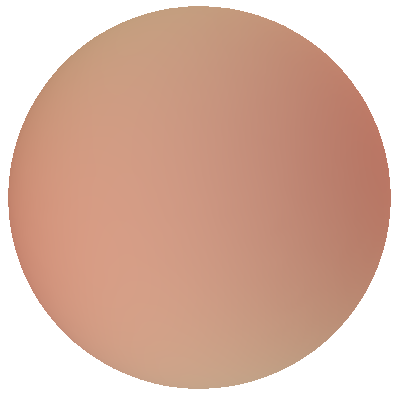
\includegraphics[width=0.2\textwidth]{Figures/chap4/illuminations/test6_FCN.png}}
	\subbottom[combination]{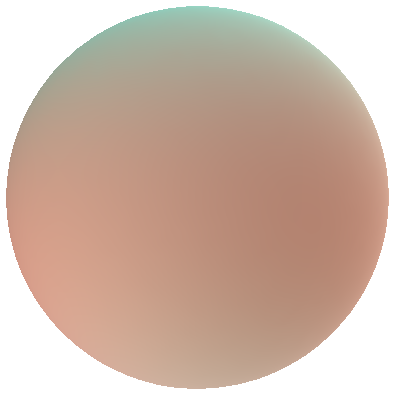
\includegraphics[width=0.2\textwidth]{Figures/chap4/illuminations/test6_combined.png}}
	\subbottom[groundtruth]{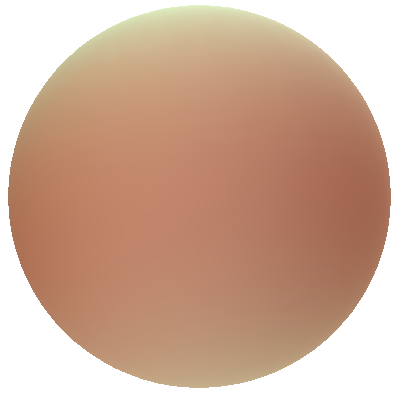
\includegraphics[width=0.2\textwidth]{Figures/chap4/illuminations/test6_groundtruth.png}}
	
	\caption{The illuminations of the last example rendered on a sphere. It seems like the illumination with the FCN mask is dull and has no specular term (only ambient). However, the illumination with the combined mask is strongly based on illumination (a).}
	\label{fig:chap4:bsp1_illumination}
\end{figure}
  
\section{Evaluation on the Original Face}
Because we showed in \Cref{sec:Oversegmentation} that the iterative algorithm of Egger et al tends to oversegment and labels skin-parts other than the face, we repeat the experiment with a rendering that shows ears, hairline, and neck too - the 'bfm' version of the Basel Face Model.

\begin{figure}
\centering
\subbottom[initial mask of the FCN]{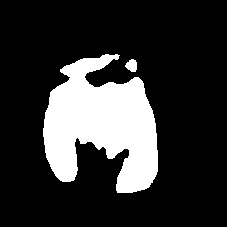
\includegraphics[width=0.24\textwidth]{Figures/chap3/hands_test0_mask_FCN_.png}\label{fig:chap4:bsp2_mask_FCN}}
\subbottom[segmentation of Egger et al]{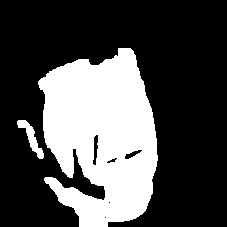
\includegraphics[width=0.24\textwidth]{Figures/chap3/hands_test0_mask_EGGER_.png}\label{fig:chap4:bsp2_mask_EGGER}}
\subbottom[combined segmentation]{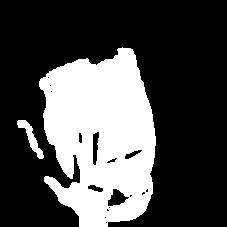
\includegraphics[width=0.24\textwidth]{Figures/chap4/hands_setting2_test0_mask_combined.png}\label{fig:chap4:bsp2_mask_combined}}
\subbottom[fit with the combined mask (Subfigure (c))]{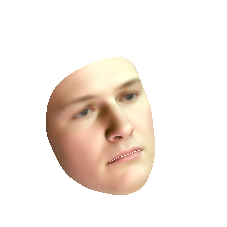
\includegraphics[width=0.24\textwidth]{Figures/chap4/hands_setting2_test0_fit_combined.png}\label{fig:chap4:bsp2_fit_combined}}
\caption{An example of the combination of the two masks. [Figure \ref{fig:chap4:bsp2_mask_FCN}] shows the segmentation of the FCN while [Figure \ref{fig:chap4:bsp2_mask_EGGER}] shows the segmentation by Egger et al. The combination is depicted in [Figure \ref{fig:chap4:bsp2_mask_combined}]. The target image for this example is the same as in [Figure \ref{fig:chap3:hands_setting2_occluded}]. [Figure \ref{fig:chap4:bsp2_fit_combined}] shows the resulting fit with the combined mask.}
\label{fig:chap4:bsp2}
\end{figure}



\pgfplotsset{height=7.5cm,width=8.5cm,compat=1.9}
\begin{figure}
	\begin{center}
		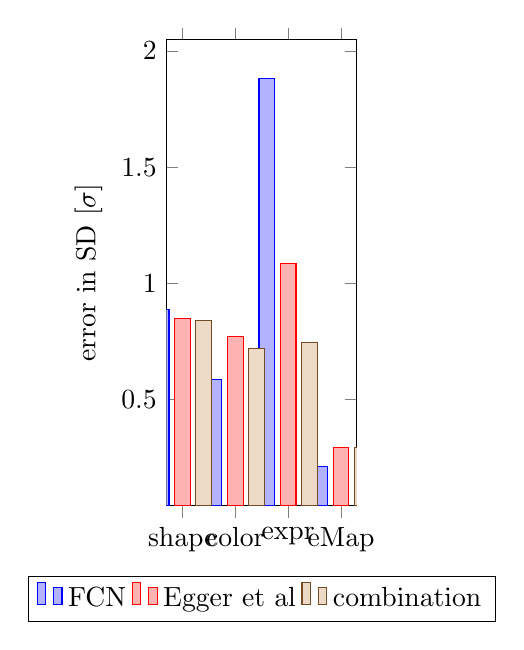
\begin{tikzpicture} 
		\begin{axis}[ 
		ybar,
		bar width=0.2cm,
		enlargelimits=0.1, 
		legend style={at={(0.5,-0.15)}, anchor=north,legend columns=-1}, 
		ylabel={error in SD [$\sigma$]},
		symbolic x coords={shape,color,expr,eMap}, 
		xtick=data,
		%nodes near coords, 
		%nodes near coords align={vertical}, 
		] 
		
		\addplot coordinates {(shape,0.8878) (color,0.5868) (expr,1.8812) (eMap,0.2104)}; 
		\addplot coordinates {(shape,0.8489) (color,0.7704) (expr,1.0859) (eMap,0.2927)}; 
		\addplot coordinates {(shape,0.8397) (color,0.7218) (expr,0.7472) (eMap,0.2927)}; 
		
		\legend{FCN, Egger et al, combination}
		\end{axis} 
		\end{tikzpicture}
		\pgfplotsset{height=7.5cm,width=4cm,compat=1.9}
		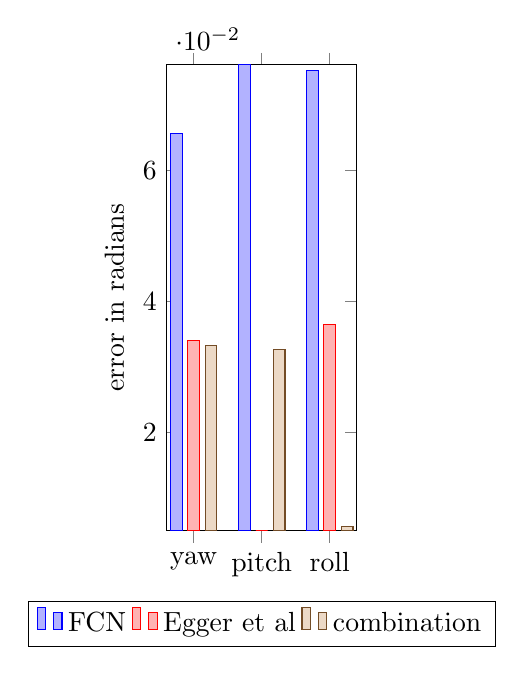
\begin{tikzpicture} 
		\begin{axis}[ 
		ybar,
		bar width=0.15cm,
		%enlarge limits=0.05,
		enlarge y limits=0.00,
		enlarge x limits=0.2,
		legend style={at={(0.5,-0.15)}, anchor=north,legend columns=-1}, 
		ylabel={error in radians},
		symbolic x coords={yaw,pitch,roll}, 
		xtick=data,
		] 
		
		\addplot coordinates {(yaw,0.0657) (pitch,0.0762) (roll,0.0753)}; 
		\addplot coordinates {(yaw,0.0341) (pitch,0.0050) (roll,0.0365)}; 
		\addplot coordinates {(yaw,0.0333) (pitch,0.0327) (roll,0.0057)}; 
		
		\legend{FCN, Egger et al, combination}
		\end{axis} 
		\end{tikzpicture}
	\end{center}
	\caption{A comparison of the Basel Face Model parameters. In this plot, the fits with the masks of Egger, of the FCN [Figure \ref{fig:chap3:zlabelsandfits_setting2}], and the fit with the combined mask [\Cref{fig:chap4:bsp1_fit_combined}] are compared. For each parameter, all dimensions are considered. With the combined segmentation, the fit is a tiny bit better than with the segmentation of Egger et al alone.}
	\label{fig:chap4:fit_comparison_2}
\end{figure}

\begin{figure}
	\centering
	\subbottom[Egger et al]{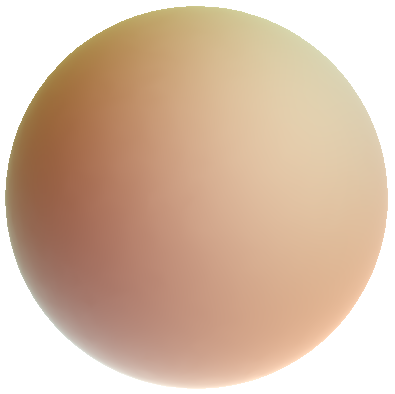
\includegraphics[width=0.24\textwidth]{Figures/chap4/illuminations/test0_EGGER.png}}
	\subbottom[FCN]{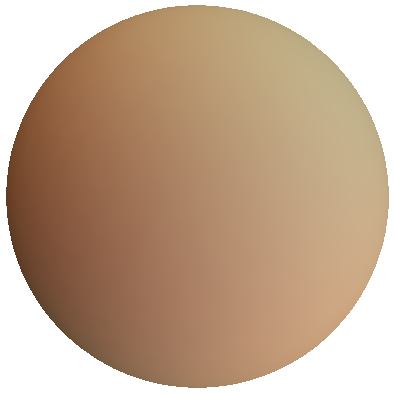
\includegraphics[width=0.24\textwidth]{Figures/chap4/illuminations/test0_FCN.png}}
	\subbottom[combination]{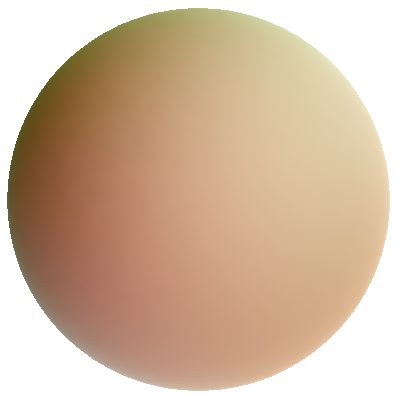
\includegraphics[width=0.24\textwidth]{Figures/chap4/illuminations/test0_combined.png}}
	\subbottom[groundtruth]{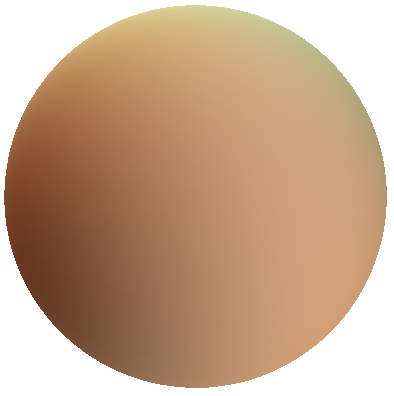
\includegraphics[width=0.24\textwidth]{Figures/chap4/illuminations/test0_groundtruth.png}}
	
	\caption{The illuminations of the last example rendered on a sphere. It seems like (as in the previous example) the illumination with the FCN mask is dull and has no specular term (only ambient). Again, the illumination with the combined mask is strongly based on illumination (a).}
	\label{fig:chap4:bsp2_illumination}
\end{figure}


